\documentclass[12pt]{book}
\usepackage[utf8]{inputenc}
\usepackage[T1]{fontenc}
\usepackage{lmodern}        % Fuentes vectoriales Type 1 (igual que Cap 3)
\usepackage{microtype}      % Mejora la legibilidad
\usepackage[spanish,es-nodecimaldot]{babel}
\usepackage[margin=2.5cm]{geometry}
\usepackage{amsmath}
\usepackage{amssymb}
\usepackage{graphicx}
\graphicspath{{imagenes/}}
\usepackage{booktabs}
\usepackage{tabularx}
\usepackage{sidecap}
\usepackage{threeparttable}
\usepackage{enumitem}
\usepackage{mathptmx}
\usepackage{url}

\AtBeginDocument{\shorthandoff{"}}

\setcounter{chapter}{12}

\begin{document}

\chapter{Sistemas de Retroalimentación y Control}
\label{chap:13}


% ---- Bloque 1: temp_cap_13_pag_873_880.tex ----
Resumen. Se presentan los fundamentos de los sistemas de retroalimentación y control, junto con su funcionamiento en personas sanas y enfermas. Los ejemplos específicos incluyen la regulación y el control de la temperatura corporal y la presión arterial, incluso durante el ejercicio, y del tamaño de la pupila.

Controlamos conscientemente nuestros procesos de pensamiento para lograr objetivos físicos, en parte mediante el uso de nuestros sentidos para proporcionar respuesta para la retroalimentación y así controlar nuestras acciones. Por ejemplo, cuando colocamos un objeto sobre una mesa, controlamos nuestras acciones utilizando nuestros ojos para proporcionar retroalimentación sobre las posiciones relativas del objeto y la mesa a medida que se acerca a ella, y nuestro sentido del tacto para proporcionar retroalimentación cuando lo colocamos sobre la mesa. Dicha retroalimentación y control también es importante en todos los procesos de fabricación. Nuestros cuerpos funcionan increíblemente bien debido a constantes procesos de retroalimentación y control.

Un sistema de retroalimentación y control muy esencial es la homeostasis, que técnicamente es la estabilidad de las condiciones químicas y físicas del líquido que rodea a las células del cuerpo. Este líquido extracelular constituye aproximadamente un tercio del líquido corporal total, e incluye el plasma sanguíneo y el líquido intersticial (el líquido tisular que se encuentra en los espacios entre las células). Los otros dos tercios del líquido son intracelulares. El líquido extracelular se controla para regular (a) la temperatura corporal, (b) la presión en los vasos sanguíneos, (c) las concentraciones de oxígeno y dióxido de carbono, (d) el pH, (e) las concentraciones de iones, como $\text{Na}^+$, $\text{K}^+$ y $\text{Ca}^{2+}$, (f) el volumen, (g) la osmolalidad (relación agua/partículas disueltas) y (h) las concentraciones de nutrientes orgánicos, como la glucosa.

Tenemos muchos otros sistemas de control importantes. Los iris de nuestros ojos se abren y se cierran en respuesta a los niveles de luz. Los músculos ciliares controlan la distancia focal de los cristalinos en nuestros ojos para enfocar objetos (acomodación, Fig. 11.22). La fuerza que utilizamos para agarrar objetos depende de la retroalimentación de la fuerza normal que obtenemos de ellos (y si el objeto «cede», aplicamos menos fuerza). Durante el ejercicio, los músculos intercostales y abdominales que controlan la respiración están regulados por el cerebro, el cual recibe información de los receptores químicos en la sangre, receptores mecánicos y metabólicos en los músculos esqueléticos, así como de receptores en los pulmones (Fig. 13.1). De manera similar, durante el ejercicio el cerebro recibe información del corazón y los músculos y luego envía señales para controlar el corazón y los vasos sanguíneos para aumentar el gasto cardíaco y la presión arterial (Fig. 13.6 abajo). El equilibrio de calor corporal y la temperatura también se controlan durante el ejercicio (Fig. 13.4 abajo). Por supuesto, estos sistemas de control también son esenciales durante el reposo. Para discusiones generales sobre dichos sistemas de control y el control en el cuerpo, véase [1, 4, 6, 7, 10, 12, 15, 19, 21].

\begin{figure}[htbp]
  \centering
  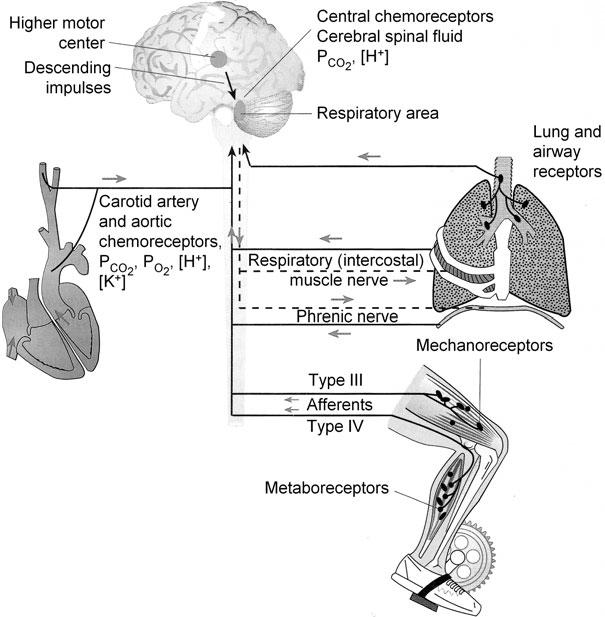
\includegraphics[width=0.55\textwidth]{131.png}
  \caption{Control del sistema respiratorio (ventilación) durante el ejercicio. El área respiratoria en el cerebro recibe señales de la región motora del cerebro, quimiorreceptores centrales y otros receptores, incluidos los quimiorreceptores de la arteria carótida y de la aorta, receptores de los músculos intercostales de los pulmones y del diafragma, y receptores mecánicos y metabólicos de los músculos esqueléticos. Durante el ejercicio, esto da como resultado un aumento de la actividad neural hacia los músculos intercostales y el diafragma a través de los nervios frénicos e intercostales. Esto aumenta la frecuencia y la profundidad de la respiración, lo que regula el oxígeno arterial, el dióxido de carbono y el pH (De [4]. Utilizado con permiso).}
  \label{fig:131}
\end{figure}

\section{Conceptos básicos de retroalimentación y control}
\label{sec:13.1}

La Figura 13.2 es un diagrama de bloques que representa la retroalimentación y el control. Hay un sensor o receptor que mide una cantidad (estímulo), como la presión arterial mediante barorreceptores. La señal de este receptor se transmite a un centro de integración, como la transmisión de señales desde los centros sensoriales al cerebro por medio de nervios. El centro de integración induce un efecto. Esta respuesta se transmite por los nervios (vías motoras) a un centro de control del efector. Existe algún efecto o respuesta de interés, como cambiar la frecuencia cardíaca o el volumen de eyección para cambiar la presión arterial. El éxito de este control se determina midiendo la respuesta, la nueva presión arterial, lo cual proporciona retroalimentación para el control.

\begin{figure}[htbp]
  \centering
  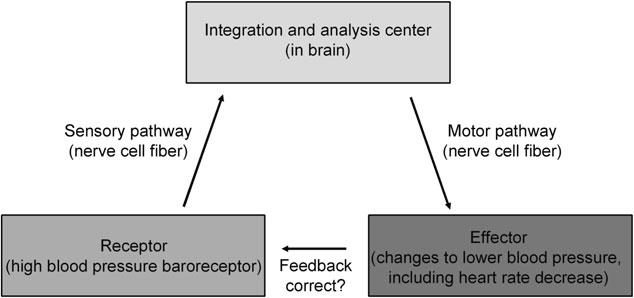
\includegraphics[width=0.8\textwidth]{132.png}
  \caption{Retroalimentación y control en el cuerpo, con un ejemplo de control de la presión arterial alta entre paréntesis (Basado en [19]).}
  \label{fig:132}
\end{figure}

La retroalimentación negativa invierte la dirección del cambio de una variación, para mantener el parámetro medido cerca del punto de consigna deseado. Este tipo de retroalimentación es muy común en el cuerpo. Generalmente existe un rango de operación centrado alrededor de este punto de consigna delimitado por valores permitidos. La Figura 13.3a muestra que el efector se activa para corregir el parámetro cuando este se desvía por encima del valor más alto permitido o por debajo del valor más bajo permitido. Los termostatos de las habitaciones suelen funcionar de la misma manera, con un rango de operación de varios grados alrededor del punto de consigna; nuestros cuerpos también tienen termostatos.

La retroalimentación positiva hace que el efector produzca un mayor cambio en la misma dirección en la que el parámetro ya está cambiando, como en la Fig. 13.3b. Este tipo de retroalimentación es poco común en el cuerpo. Un ejemplo es la lactancia, que conduce a la producción de más leche en las madres. Otro ocurre durante las etapas finales de la muerte por insuficiencia cardíaca congestiva crónica [16]. Con esta condición, el músculo cardíaco no es capaz de contraerse lo suficiente para alcanzar el volumen de eyección necesario. El líquido se acumula en las venas, causando un aumento de la presión en los pulmones y otros órganos y no circula suficiente sangre a los órganos. En lugar de devolver el sistema a un punto de consigna mejor, la retroalimentación positiva empeora el rendimiento del corazón y, lo que es igual de perjudicial, hace que el volumen sanguíneo aumente de forma constante mucho más allá del valor óptimo. El mal rendimiento cardíaco conduce al engrosamiento del músculo cardíaco, pero el nuevo músculo es de baja calidad y disminuye aún más el rendimiento cardíaco. El ya limitado flujo de sangre al músculo cardíaco se vuelve cada vez más insuficiente para mantener saludable la mayor cantidad de músculo, lo que deteriora aún más el rendimiento. Simultáneamente, el volumen sanguíneo aumenta, incrementando la carga sobre el corazón dañado, debido a la respuesta de los riñones. Los riñones filtran parte de la sal y el agua y normalmente los eliminan de la circulación. Para una persona sana, esto mantiene el volumen sanguíneo general. Para alguien con insuficiencia cardíaca congestiva, dicha eliminación disminuiría un poco el volumen sanguíneo y reduciría la carga sobre el corazón, lo cual sería bueno. Sin embargo, los riñones detectan el menor flujo sanguíneo y, en su lugar, devuelven a la circulación la sal y el agua que han filtrado en un esfuerzo por aumentar el bajo volumen sanguíneo a niveles normales. Esto aumenta de manera indeseable el volumen sanguíneo, lo que incrementa la carga sobre el corazón, lo que hace que el corazón se deteriore más y bombee menos sangre, lo que hace que los riñones aumenten el volumen sanguíneo total, y así sucesivamente, acelerando el proceso de la muerte.

\begin{figure}[htbp]
  \centering
  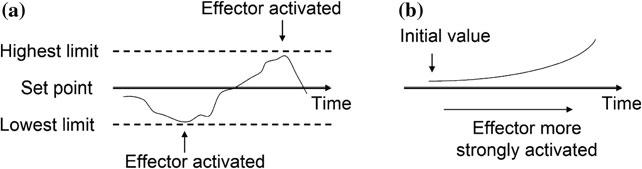
\includegraphics[width=0.8\textwidth]{133.png}
  \caption{a) Retroalimentación negativa y b) positiva (Basado en [19]).}
  \label{fig:133}
\end{figure}

\subsection{Teoría de control (Tema avanzado)}
\label{subsec:13.1.1}

Se necesita retroalimentación para controlar un parámetro $P$, como la presión arterial o la temperatura, para mantenerlo cerca de un punto de consigna $P_0$. El nivel de retroalimentación suele ser proporcional a la diferencia entre el valor actual del parámetro y el punto de consigna deseado [15]. La ganancia $g$ es el factor de proporcionalidad y determina la magnitud de la respuesta. Esta respuesta provoca un cambio $dP$ en el tiempo $dt$, por lo que
\begin{equation}
  dP = -g(P - P_0)dt. \label{eq:13.1}
\end{equation}

Esta retroalimentación no es instantánea. Se retrasa un tiempo $\tau_d$ debido a los retrasos asociados con la detección, la transmisión neuronal al cerebro, el procesamiento en el cerebro, la transmisión neuronal a los efectores y la rapidez con la que los efectores pueden provocar un cambio. En consecuencia, un cambio en el tiempo $t$ se debe a la retroalimentación proporcionada por los sensores en el tiempo $t - \tau_d$, por lo que (\ref{eq:13.1}) cambia a
\begin{equation}
  dP(t) = -g(P(t - \tau_d) - P_0)dt, \label{eq:13.2}
\end{equation}
o definiendo $p = P - P_0$
\begin{equation}
  \frac{dp(t)}{dt} = -g p(t - \tau_d). \label{eq:13.3}
\end{equation}

La respuesta deseada es una disminución de la magnitud de $p$ de forma monótona, una oscilación estable de $p$ alrededor de 0 (y por lo tanto de $P$ alrededor de $P_0$), o alguna combinación de ambas. ¿Qué valores de $g$ y $\tau_d$ pueden producir esta retroalimentación negativa estable deseada? Obviamente, $g$ debe ser positiva y puede parecer que cuanto mayor sea la ganancia mejor, pero veremos que los valores grandes de la ganancia no siempre son deseables.

Intentemos resolver (\ref{eq:13.3}) sustituyendo en ella la posible solución $p(t) = p \exp(zt)$. En general, $z$ puede ser un número complejo, con $z = x + iy$. El término imaginario $y$ proporciona un comportamiento oscilatorio alrededor del punto de consigna, mientras que $x < 0$ da un decaimiento exponencial hacia el punto de consigna y $x > 0$ da un aumento exponencial alejándose del punto de consigna, siendo este último caso indeseable. La ecuación (\ref{eq:13.3}) se convierte entonces en
\begin{equation}
  z = -g \exp(-z\tau_d). \label{eq:13.4}
\end{equation}

Pueden existir soluciones razonables para $x \le 0$. Debido a que $\exp(iq) = \cos q + i\sin q$, la ecuación (\ref{eq:13.4}) se convierte en ecuaciones separadas para las partes real e imaginaria:
\begin{equation}
  x = -g \exp(-x\tau_d) \cos(y\tau_d), \label{eq:13.5}
\end{equation}
\begin{equation}
  y = g \exp(-x\tau_d) \sin(y\tau_d). \label{eq:13.6}
\end{equation}

Estas son ecuaciones trascendentes que en general deben resolverse numéricamente. Sin embargo, seremos capaces de resolverlas analíticamente en regímenes especiales.

La solución con $x = 0$ es aquella que oscila alrededor del punto de consigna. El uso de $x = 0$ en (\ref{eq:13.5}) conduce a $0 = -g \cos(y\tau_d)$, lo que da $y = \pi/2\tau_d$. El uso de $x = 0$ en (\ref{eq:13.6}) conduce a $y = g \sin(y\tau_d)$ y, con $y = \pi/2\tau_d$, esto se convierte en $\pi/2\tau_d = g \sin((\pi/2\tau_d)\tau_d) = g$. Esto significa que
\begin{equation}
  g\tau_d = \frac{\pi}{2}, \label{eq:13.7}
\end{equation}
y, por lo tanto, si el tiempo de retraso es $\tau_d$, hay una respuesta oscilatoria cuando la ganancia es $g = \pi/2\tau_d$. Esta es una solución aceptable.

Ahora supongamos que $x$ tiene una magnitud pequeña pero no es necesariamente 0. La ecuación (\ref{eq:13.5}) todavía da $y \approx \pi/2\tau_d$ y, por lo tanto, $\sin(y\tau_d) \approx 1$. Debido a que $\exp(q) \approx 1 + q$ para $|q| \ll 1$, la ecuación (\ref{eq:13.6}) se convierte en $y \approx g(1 - x\tau_d)\sin(y\tau_d) \approx g(1 - x\tau_d)$ y, por tanto,
\begin{equation}
  x \approx \frac{1}{\tau_d} \left( 1 - \frac{\pi}{2g\tau_d} \right). \label{eq:13.8}
\end{equation}

Para $g\tau_d < \pi/2$, vemos que $x < 0$ y el parámetro $P$ se aproxima al punto de consigna como una oscilación con una magnitud que disminuye con el tiempo. Para $g\tau_d = \pi/2$, es evidente que $x = 0$ y el parámetro $P$ oscila alrededor del punto de consigna, como se mostró anteriormente. Para $g\tau_d > \pi/2$, vemos que $x > 0$ y el parámetro $P$ oscila alrededor del punto de consigna con una magnitud que aumenta con el tiempo, lo cual es inestable. Por lo tanto, este criterio de estabilidad establece un límite superior para la ganancia posible para un tiempo de retraso dado, expresado como
\begin{equation}
  g\tau_d \le \frac{\pi}{2}. \label{eq:13.9}
\end{equation}

\section{Regulación del cuerpo}
\label{sec:13.2}

\subsection{Regulación de la temperatura}
\label{subsec:13.2.1}

La regulación de la temperatura corporal está estrechamente ligada a la discusión en el Cap. 6 sobre la producción de calor por el metabolismo y los modos de pérdida de calor del cuerpo. La temperatura corporal central normal es de $37 \pm 2\ ^\circ\text{C}$ ($98.6 \pm 3.6\ ^\circ\text{F}$). Los aumentos y disminuciones grandes significan problemas. Muy por encima de las temperaturas corporales normales, a los $41\ ^\circ\text{C}$ ($106\ ^\circ\text{F}$), el sistema nervioso central comienza a deteriorarse y se producen convulsiones. A los $45\ ^\circ\text{C}$ ($115\ ^\circ\text{F}$), las proteínas se desnaturalizan, lo que es seguido por la muerte. Para temperaturas inferiores a la normal, a los $33\ ^\circ\text{C}$ ($91\ ^\circ\text{F}$), las funciones nerviosas se deprimen hasta el punto de perder el conocimiento. A los $30\ ^\circ\text{C}$ ($86\ ^\circ\text{F}$), el sistema de regulación de la temperatura falla. A los $28\ ^\circ\text{C}$ ($82\ ^\circ\text{F}$), se produce fibrilación cardíaca, lo que conduce a la muerte. El cuerpo es bastante bueno regulando la temperatura central, como se desprende de la Fig. 6.20, pero tiene sus límites y puede fallar, como es evidente en las Figs. 6.21, 6.22 y 6.23. La Figura 13.4 ilustra cómo los receptores en la piel y en el núcleo central detectan la temperatura y envían información al cerebro. Las temperaturas fuera del rango de normalidad conducen a actos conscientes y a la actividad automática del cuerpo para corregir las temperaturas.

\begin{figure}[htbp]
  \centering
  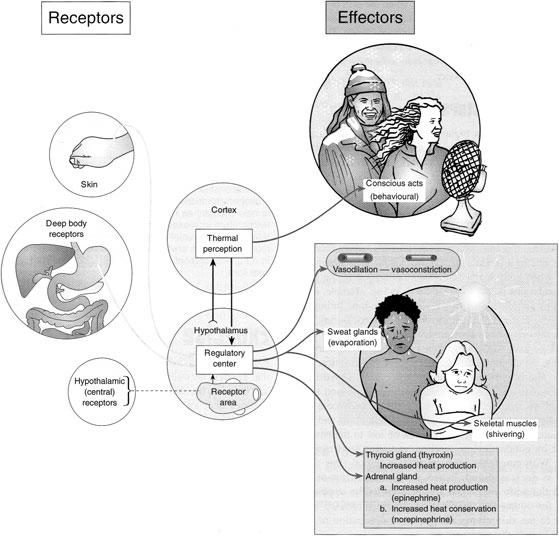
\includegraphics[width=0.55\textwidth]{134.png}
  \caption{El sistema termorregulador, que incluye la entrada al cerebro desde los receptores y la salida desde el cerebro hacia los efectores. El centro hipotalámico transmite información a los órganos efectores para estimular los procesos de producción y conservación de calor que se muestran cuando los receptores de temperatura central difieren del punto de consigna de $37\ ^\circ\text{C}$ (De [4]. Utilizado con permiso).}
  \label{fig:134}
\end{figure}

Cada persona tiene una temperatura de punto de consigna, que varía en aproximadamente $\pm0.3\ ^\circ\text{C}$ ($\pm0.5\ ^\circ\text{F}$) entre los individuos [3]. El punto de consigna medio para la temperatura de la piel es de aproximadamente $33\ ^\circ\text{C}$ ($91.4\ ^\circ\text{F}$). (En el Cap. 6 utilizamos una temperatura de la piel de $34\ ^\circ\text{C}$). Las temperaturas de la piel por encima de los $34.5\ ^\circ\text{C}$ ($94\ ^\circ\text{F}$) provocan sudoración activa, mientras que aquellas por debajo de los $30\ ^\circ\text{C}$ ($86\ ^\circ\text{F}$) conducen al aumento de la actividad metabólica asociada con los escalofríos.

Recordando nuestra discusión en el Cap. 6, la conservación de la energía implica una conservación de la generación y pérdida de calor:
\begin{equation}
  \left( \frac{dQ}{dt} \right)_{\text{neto}} = \left( \frac{dQ}{dt} \right)_{\text{metabolismo}} + \left( \frac{dQ}{dt} \right)_{\text{pérdida pasiva}} + \left( \frac{dQ}{dt} \right)_{\text{controlado por el cuerpo}}. \label{eq:13.10}
\end{equation}

El lado izquierdo es la tasa de calentamiento neta debido a todos los modos de producción y pérdida de calor. El primer término en el lado derecho es la producción de calor a partir de la actividad metabólica y la actividad física; es $>0$. El segundo término es la pérdida de calor debido a modos pasivos, tales como desde la piel, radiación, convección, etc.; es $<0$. El tercer término es el debido al calentamiento controlado por el cuerpo ($>0$) y/o la eliminación de calor ($<0$) [1].

Nuestra discusión en el Cap. 6, como en (6.5) y (6.36), nos mostró cómo cambia la temperatura corporal con un flujo neto de calor hacia adentro o hacia afuera del cuerpo, según
\begin{equation}
  \left( \frac{dQ}{dt} \right)_{\text{neto}} = C \frac{dT}{dt} = (60\ \text{kcal}/^\circ\text{C}) \frac{dT}{dt}, \label{eq:13.11}
\end{equation}
donde $C$ es la capacidad calorífica $= 60\ \text{kcal}/^\circ\text{C}$ para una persona de $70\ \text{kg}$. La capacidad calorífica $C = \text{masa}\ (=70\ \text{kg}) \times \text{calor específico}\ c\ (= 0.83\ \text{kcal}/^\circ\text{C}\cdot\text{kg})$. Sabemos que la tasa mínima de calentamiento debido al metabolismo es la BMR, por lo que se puede escribir como
\begin{equation}
  \left( \frac{dQ}{dt} \right)_{\text{metabolismo}} = f (\text{BMR}), \label{eq:13.12}
\end{equation}
donde $f$ es el factor de actividad (un multiplicador entre 1 y aproximadamente 20) y $\text{BMR} = 70\ \text{kcal/h}$.

Si no hay pérdida de calor (y los dos últimos términos de (\ref{eq:13.10}) son cero), vemos que
\begin{equation}
  C \frac{dT}{dt} = f (\text{BMR}) = f\ (70\ \text{kcal/h}), \label{eq:13.13}
\end{equation}
por lo que
\begin{equation}
  \frac{dT}{dt} = f \frac{\text{BMR}}{C} = f \frac{70\ \text{kcal/h}}{60\ \text{kcal}/^\circ\text{C}} = 1.2 f\ ^\circ\text{C/h}. \label{eq:13.14}
\end{equation}

Esto es similar a (6.36). Sin medios adecuados de pérdida de calor, no sobreviviríamos por mucho tiempo a un ejercicio pesado. Con $f = 20$ para ejercicio pesado, vemos que $dT/dt = 24\ ^\circ\text{C/h}$.

Consideremos ahora lo que sucede cuando existe únicamente pérdida pasiva de calor, debido a radiación y convección, sin control. A partir de (\ref{eq:13.10}), la pérdida de calor debido a radiación y convección es
\begin{equation}
  \left( \frac{dQ}{dt} \right)_{\text{pérdida pasiva}} = -(A h_r + A h_c)(T_{\text{piel}} - T_{\text{hab}}) = -\lambda (T_{\text{piel}} - T_{\text{hab}}), \label{eq:13.15}
\end{equation}
donde $\lambda = A(h_r + h_c)$. Para una persona con un área corporal de $1.5\ \text{m}^2$, el parámetro de radiación $A h_r \sim 12\ \text{kcal}/(\text{h}\cdot^\circ\text{C})$. El parámetro de convección es $A h_c \sim 13\ \text{kcal}/(\text{h}\cdot^\circ\text{C})$ para una persona desnuda en presencia de una velocidad del viento de $9\ \text{m/s}$. Esto es mucho más alto que los valores típicos para personas vestidas. Para una persona desnuda en una brisa de $15\ \text{m/s}$, es mayor por un factor de 5 que el valor utilizado aquí.

La ecuación (\ref{eq:13.15}) se convierte ahora en
\begin{equation}
  C \frac{dT}{dt} = f(\text{BMR}) - \lambda (T_{\text{cuerpo}} - T_{\text{hab}}) \label{eq:13.16}
\end{equation}
o
\begin{equation}
  (60\ \text{kcal}/^\circ\text{C}) \frac{dT}{dt} = f(70\ \text{kcal/h}) - (25\ \text{kcal/h}\cdot^\circ\text{C})(T_{\text{cuerpo}} - T_{\text{hab}}), \label{eq:13.17}
\end{equation}
donde hemos llamado $T_{\text{cuerpo}}$ a la temperatura del cuerpo y ahora ignoramos las diferencias entre las temperaturas de la piel y central. Estas ecuaciones se pueden resolver sustituyendo la forma
\begin{equation}
  T_{\text{cuerpo}}(t) = \alpha + \beta \exp(-t/\tau_r), \label{eq:13.18}
\end{equation}
donde $\tau_r$ es el tiempo de respuesta característico. Esta sustitución da
\begin{equation}
  C\beta(-1/\tau_r) \exp(-t/\tau_r) = f(\text{BMR}) - \lambda(\alpha + \beta \exp(-t/\tau_r) - T_{\text{hab}}) \label{eq:13.19}
\end{equation}
\begin{equation}
  = f(\text{BMR}) - \lambda(\alpha - T_{\text{hab}}) - \lambda\beta \exp(-t/\tau_r). \label{eq:13.20}
\end{equation}

Debido a que esto debe ser válido para todo tiempo $t$, podemos igualar los coeficientes de los términos $\exp(-t/\tau_r)$ para obtener
\begin{equation}
  C\beta(-1/\tau_r) = -\lambda\beta, \label{eq:13.21}
\end{equation}
\begin{equation}
  \tau_r = \frac{C}{\lambda} = \frac{60\ \text{kcal}/^\circ\text{C}}{25\ \text{kcal/h}\cdot^\circ\text{C}} = 2.4\ \text{h}, \label{eq:13.22}
\end{equation}

% Control de Calidad: 37 párrafos origen -> 37 párrafos salida. Mapeo 1:1 verificado. Sin omisiones.

% ---- Bloque 2: temp_cap_13_pag_881_888.tex ----
y luego igualar los términos constantes para obtener
\begin{equation}
  f (\text{BMR}) = \lambda(\alpha - T_{\text{hab}}), \label{eq:13.23}
\end{equation}
o
\begin{equation}
  \alpha = T_{\text{hab}} + \frac{f \text{BMR}}{\lambda} = T_{\text{hab}} + f \frac{70\ \text{kcal/h}}{25\ \text{kcal/h}\cdot^\circ\text{C}} = T_{\text{hab}} + 2.8 f\ ^\circ\text{C}. \label{eq:13.24}
\end{equation}

En $t = 0$ llamaremos $T_{\text{cuerpo}}(t = 0) = T_{\text{cuerpo, inicial}}$ (que es la condición inicial), por lo que
\begin{equation}
  T_{\text{cuerpo}}(0) = T_{\text{cuerpo, inicial}} = \alpha + \beta \label{eq:13.25}
\end{equation}
y por lo tanto
\begin{equation}
  \beta = T_{\text{cuerpo, inicial}} - \alpha = T_{\text{cuerpo, inicial}} - T_{\text{hab}} - 2.8 f\ ^\circ\text{C}. \label{eq:13.26}
\end{equation}

La solución final es
\begin{equation}
  T_{\text{cuerpo}}(t) = T_{\text{hab}} + 2.8 f\ ^\circ\text{C} + (T_{\text{cuerpo, inicial}} - T_{\text{hab}} - 2.8 f\ ^\circ\text{C}) \exp(-t/\tau_r). \label{eq:13.27}
\end{equation}

Este es un ejemplo de calentamiento en bucle abierto (o ciclo abierto), porque no hay retroalimentación ni control. Los problemas en este sistema de regulación de la temperatura son evidentes a partir de (\ref{eq:13.27}). La temperatura final en estado estacionario (es decir, para $t \gg \tau_r = 2.4\ \text{h}$) es
\begin{equation}
  T_{\text{cuerpo, estado estacionario}} = T_{\text{hab}} + \frac{f \text{BMR}}{\lambda} = T_{\text{hab}} + 2.8 f\ ^\circ\text{C}. \label{eq:13.28}
\end{equation}

Si $T_{\text{hab}} = 21\ ^\circ\text{C}$ ($69.8\ ^\circ\text{F} \approx 70\ ^\circ\text{F}$) y estuviéramos en reposo, de modo que $f \sim 1$, nuestra temperatura corporal en estado estacionario sería de $\approx 24\ ^\circ\text{C}$ ($75\ ^\circ\text{F}$), que es mucho menor que nuestra temperatura corporal deseada. Si estuviéramos haciendo ejercicio bastante duro, de modo que $f = 10$, nuestra temperatura corporal en estado estacionario sería de $\approx 49\ ^\circ\text{C}$ ($120\ ^\circ\text{F}$), que es demasiado alta. Podríamos cambiar conscientemente $\lambda$ un poco (a través de $h_c$: disminuyéndola al ponernos ropa pesada en el primer caso o aumentándola al aumentar la velocidad del viento sobre nuestros cuerpos desnudos en el segundo caso), y esto ayudaría un poco. Idealmente, querríamos fijar
\begin{equation}
  T_{\text{cuerpo, estado estacionario}} - T_{\text{hab}} = 37\ ^\circ\text{C}\ (98.6\ ^\circ\text{F}) - 21\ ^\circ\text{C}\ (69.8\ ^\circ\text{F}) = 16\ ^\circ\text{C}\ (28.8\ ^\circ\text{F}) \label{eq:13.29}
\end{equation}
\begin{equation}
  = \frac{f \text{BMR}}{\lambda} = 2.8 f\ ^\circ\text{C}, \label{eq:13.30}
\end{equation}
por lo que $f \sim 6$ con nuestra $\lambda$ actual. Podríamos regular la temperatura cambiando $f$ o $\lambda$. Esto significa que para mantener nuestra temperatura corporal tendríamos que realizar constantemente actividades moderadas, como natación lenta (para la misma $\lambda$). Si nos abrigáramos un poco (disminuyendo $\lambda$), podríamos reducir $f$ un poco, por ejemplo a $f = 4$, lo que significaría que aún tendríamos que realizar actividades, como caminar moderadamente rápido, incluso mientras dormimos (como el sonambulismo constante).

Otra característica negativa de las consecuencias de (\ref{eq:13.27}) es que tiene una constante de tiempo $\tau_r = 2.4\text{ h}$ que es demasiado larga. Si decidiéramos cambiar nuestro nivel de actividad (y por lo tanto cambiar $f$), nuestra temperatura corporal tardaría unas $5\text{ h}$ en estabilizarse a la nueva temperatura en estado estacionario; esto no es razonable. Estos resultados aparentemente ridículos no pueden atribuirse a las suposiciones que hemos hecho en los términos de ganancia y pérdida de calor hasta ahora. Hemos omitido el último término de (\ref{eq:13.10}), que describe la retroalimentación y el control para la regulación de temperatura en bucle cerrado (o ciclo cerrado). Necesitamos esto para mantener la temperatura corporal dentro del rango normal.

El último término de (\ref{eq:13.10}) $(dQ/dt)_{\text{controlado por el cuerpo}}$ describe las respuestas involuntarias del cuerpo para mantener una temperatura corporal normal, que podemos llamar el punto de consigna: la temperatura objetivo. Cuando se necesita un aumento de temperatura, este término es positivo debido al incremento de la actividad metabólica y la actividad motora, como los escalofríos (hasta la tasa metabólica máxima o de cumbre, Cap. 6); este calor va directamente al núcleo central y a los músculos. Cuando se necesita una disminución de temperatura, este término de control es negativo, por ejemplo, debido a la sudoración. El cuerpo puede perder $1\text{ L/h}$ de agua por sudoración; si todo este sudor se evapora (y no se limpia), entonces, con el calor de evaporación del agua de $540\text{ kcal/L}$, la pérdida de calor por sudoración puede ser de $540\text{ kcal/h}$. Mediante el control vasomotor, este término de control puede ser positivo o negativo. Si la sangre se dirige a los vasos más cercanos a la piel, el enfriamiento es más eficaz y el último término de (\ref{eq:13.10}) es negativo. Si la sangre se desvía a los vasos más alejados de la piel y más cercanos al núcleo, el enfriamiento es menos eficaz y el término de control es positivo. Una razón por la que el enfriamiento es menos eficaz es el mecanismo de intercambio de calor a contracorriente descrito en la Fig. 6.19.

La Figura 13.5 muestra la tasa de pérdida de calor debido a la sudoración en función de la temperatura corporal central. Esta pérdida es cero cuando el núcleo está más frío de lo normal y aumenta de forma bastante lineal con la temperatura como $K_{\text{sudor}}(T_{\text{cuerpo}} - 36.85\ ^\circ\text{C})$ donde $K_{\text{sudor}} \sim 750\ \text{kcal/}(\text{h}\cdot^\circ\text{C})$, cuando el núcleo está más caliente de lo normal (para temperaturas de la piel entre 33 y $38\ ^\circ\text{C}$). Ahora (\ref{eq:13.10}) se convierte en

\begin{SCfigure}[0.9][htbp]
  \centering
  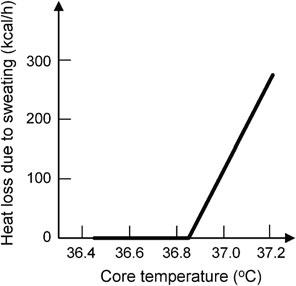
\includegraphics[width=0.5\textwidth]{135.png}
  \caption{Tasa de pérdida de calor debido a la sudoración, para temperaturas de la piel entre 33 y $38\ ^\circ\text{C}$ (Basado en [1, 2]).}
  \label{fig:135}
\end{SCfigure}

\begin{equation}
  C \frac{dT}{dt} = f P_0 - \lambda(T_{\text{cuerpo}} - T_{\text{hab}}) - K_{\text{sudor}}(T_{\text{cuerpo}} - 36.85\ ^\circ\text{C}), \label{eq:13.31}
\end{equation}
o
\begin{equation}
  \begin{split}
    (60\ \text{kcal}/^\circ\text{C}) \frac{dT}{dt} = {}& f (70\ \text{kcal/h}) - (25\ \text{kcal/h}\cdot^\circ\text{C})(T_{\text{cuerpo}} - T_{\text{hab}}) \\
    & - (750\ \text{kcal/h}\cdot^\circ\text{C})(T_{\text{cuerpo}} - 36.85\ ^\circ\text{C}).
  \end{split}
  \label{eq:13.32}
\end{equation}

Téngase en cuenta que $T_{\text{cuerpo}}$ en el término de pérdida pasiva de calor realmente se refiere a la temperatura de la piel, mientras que en el término de control es la temperatura central. La solución de esta ecuación tiene una forma similar a (\ref{eq:13.27}) con el tiempo de respuesta
\begin{equation}
  \tau_r = \frac{C}{\lambda + K}. \label{eq:13.33}
\end{equation}

Dado que $K/\lambda = 30$, la constante de tiempo es ahora menor por un factor de 31, dando $2.4\text{ h}/31 \approx 4.7\text{ min}$, lo cual es mucho más razonable.

Nótese que hemos podido ver cómo el cuerpo puede aumentar la ganancia para producir un tiempo de respuesta que es razonable en una escala de tiempo fisiológica. Hemos ignorado la cuestión del tiempo de retraso $\tau_d$, como se discutió en la sección anterior. Para este proceso, al menos $\tau_d \ll \tau_r$ y, por lo tanto, el tiempo de retraso no es importante aquí.

Nuestros cuerpos suelen tener un punto de consigna para la temperatura central de unos $37\ ^\circ\text{C}$. A veces, cuando estamos enfermos, unas toxinas bacterianas llamadas pirógenos aumentan este punto de consigna. Cuando este punto de consigna aumenta, sentimos frío hasta que nuestras acciones voluntarias e involuntarias hacen que nuestra temperatura aumente a este nuevo nivel. Podemos disminuir la pérdida de calor cubriéndonos con mantas (lo cual es voluntario) y disminuir el flujo de sangre a la piel (involuntario). Podemos aumentar nuestra tasa metabólica mediante escalofríos (involuntario). Como se señaló en el Cap. 6, la anestesia puede afectar el mecanismo de regulación de la temperatura del cuerpo [5].

Las mujeres tienden a preferir temperaturas ambiente más altas que los hombres, hasta en $\approx 3\ ^\circ\text{C}$, a pesar de que tanto hombres como mujeres se sienten térmicamente cómodos con la misma temperatura promedio de la piel, $\approx 33\ ^\circ\text{C}$. En las oficinas con aire acondicionado, las temperaturas se establecen sobre la base de modelos que utilizan las tasas metabólicas en reposo más altas de los hombres, por lo que las mujeres tienden a sentir frío en dichas oficinas [8, 13, 14, 20].

Con la edad avanzada, hay una menor producción metabólica de calor y vasoconstricción periférica en respuesta a las bajas temperaturas ambientales, y una menor producción de sudor y flujo sanguíneo en la piel, y un mayor gasto cardíaco en respuesta a las altas temperaturas ambientales. Sin embargo, el sistema de regulación de la temperatura no se ve muy comprometido con la edad avanzada, después de contabilizar los efectos de las enfermedades crónicas y el estilo de vida más sedentario [11].

\subsection{Control de la presión arterial}
\label{subsec:13.2.2}

El cerebro recibe continuamente información del corazón y de los músculos y luego envía señales para controlar el corazón y los vasos sanguíneos para regular la presión arterial (Fig. 13.6). Por ejemplo, los barorreceptores del seno carotídeo (sensores de presión en la arteria carótida) emiten una señal que se transmite por el nervio del seno carotídeo que va al cerebro [18]. La frecuencia de esta señal $F$ es aproximadamente proporcional a la cantidad en que la presión arterial ---detectada por los barorreceptores $p_b$--- supera a una presión umbral $p_t$, y esta dependencia se ha modelado como

\begin{figure}[htbp]
  \centering
  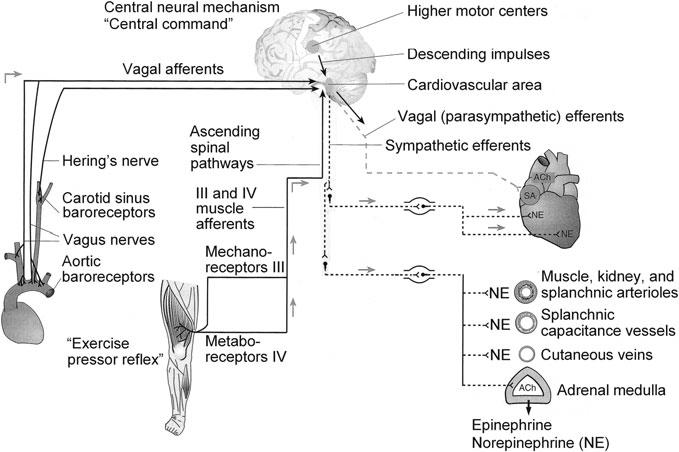
\includegraphics[width=0.7\textwidth]{136.png}
  \caption{Control del sistema cardiovascular durante el ejercicio, mostrando las entradas de control a la izquierda y las salidas a la derecha. Los impulsos nerviosos de la región motora del cerebro en el cerebro y la entrada aferente de los barorreceptores arteriales y los receptores de los músculos esqueléticos convergen en la región cardiovascular de la médula en el cerebro. Durante el ejercicio, esto da como resultado una reducción de la actividad parasimpática hacia el corazón y un aumento de la actividad simpática hacia el corazón, los vasos sanguíneos y la médula suprarrenal. (Los sistemas nerviosos parasimpático y simpático son sistemas de regulación automática que, respectivamente, «relajan» y «presionan» los sistemas, como los órganos, en el cuerpo). Esto conduce a un aumento de la presión arterial y del gasto cardíaco (De [4]. Utilizado con permiso).}
  \label{fig:136}
\end{figure}

\begin{equation}
  F + K_1 \frac{dF}{dt} = K_2(p_b - p_t) + K_3 \frac{dp_b}{dt}, \label{eq:13.34}
\end{equation}
donde $K_1$, $K_2$ y $K_3$ son constantes. Nótese la similitud de esta ecuación con la que describe el modelo de Kelvin de las propiedades mecánicas de los materiales (4.68). La frecuencia no es directamente proporcional al exceso de presión debido a los dos términos derivados. El término $dp_b/dt$ describe el sobreimpulso observado en la frecuencia.

El término $dF/dt$ describe cómo las tasas de disparo del receptor continúan cambiando incluso después de que la presión se ha estabilizado.

En el sistema de retroalimentación general, se observa una disminución de la presión arterial $\Delta p_a$ en respuesta a un cambio en la presión en los barorreceptores $\Delta p_b$, la cual viene dada por
\begin{equation}
  \Delta p_a = -g \Delta p_b, \label{eq:13.35}
\end{equation}
donde $g$ es el factor de ganancia. Una expresión más exacta es
\begin{equation}
  \Delta p_a = -g \Delta p_b - K_4 \frac{dp_b^+}{dt}, \label{eq:13.36}
\end{equation}
donde el último término denota la tasa de cambio de presión solo cuando está aumentando ($p_b^+$). Se ha medido que el factor de ganancia de bucle abierto $g_o$ varía de 2 a 9 en perros y humanos en sistemas aislados sin retroalimentación. El factor en un sistema de bucle cerrado con retroalimentación $g_c$ puede ser menor; en particular, el cuerpo lo reduce durante una hemorragia.

\subsection{Regulación durante el ejercicio}
\label{subsec:13.2.3}

Varias funciones y propiedades del cuerpo están bajo control activo durante el ejercicio. Los barorreceptores arteriales y los mecanorreceptores de los músculos esqueléticos son entradas para el área cardiovascular de la médula en el cerebro, junto con los impulsos de la región motora del cerebro, para regular el sistema cardiovascular (Fig. 13.6). Esto resulta en actividad simpática en el corazón, los vasos sanguíneos y la médula suprarrenal, lo que conduce a aumentos en la presión arterial y el gasto cardíaco.

Para que este aumento del flujo sanguíneo sea útil, debe haber un aumento concomitante en la entrada de aire y, por lo tanto, el control del sistema de ventilación es vital (Fig. 13.1). Además de las señales utilizadas para el control cardiovascular, existen señales de receptores que controlan los componentes respiratorios, como los músculos intercostales y el diafragma. Esto da como resultado actividad neural para aumentar la frecuencia y la profundidad de la respiración, lo que regula el $\text{O}_2$, $\text{CO}_2$ y el pH arteriales. (Véase [9, 10] para un modelo de respiración). Por supuesto, durante el ejercicio el cuerpo debe controlar la temperatura (Fig. 13.4).

Durante el ejercicio, la tasa de metabolismo aumenta y el cuerpo debe perder calor de forma activa. Esto ocurre a través del sistema de control de temperatura, descrito anteriormente y en la Fig. 13.4.

\subsection{Regulación del tamaño de la pupila}
\label{subsec:13.2.4}

El tamaño de la pupila de un ojo y el reflejo de la pupila están controlados por las contracciones del músculo constrictor pupilar, dispuesto circularmente, y del músculo dilatador pupilar, dispuesto radialmente [10]. Esta regulación está controlada por el flujo de luz (luminoso) a través de la pupila $\phi = I A$, donde $I$ es la iluminancia sobre el ojo y $A$ es el área de la pupila. En estado estacionario, cuanto mayor es $I$, menor se vuelve $A$, por lo que este es un ejemplo de retroalimentación negativa. Sin embargo, esta retroalimentación ocurre después de un tiempo de retraso o latencia de $\tau \sim 180\text{--}400\ \text{ms}$, debido a los tiempos de retraso en la transmisión nerviosa desde la retina al cerebro, el análisis en el cerebro, la transmisión nerviosa desde el cerebro a estos músculos y la activación de los músculos.

Podemos modelar esta actividad muscular $x(t)$ relacionándola con la tasa de llegada de potenciales de acción desde el cerebro $R(t)$
\begin{equation}
  \tau_x \frac{dx(t)}{dt} + x(t) = R(t), \label{eq:13.37}
\end{equation}
donde $\tau_x$ es este tiempo de respuesta específico. Se sabe que $R(t)$ es cero por debajo de un umbral de flujo de luz dado $\phi_{\text{umbral}}$ y aumenta logarítmicamente con el flujo por encima de este umbral, para este flujo un tiempo $\tau$ antes, $\phi(t - \tau) = I(t - \tau) A(t - \tau)$. Por lo tanto, $R(t)$ es proporcional a $F(u)$, con $F(u) = u$ para $u > 0$ y $= 0$ para $u \le 0$, donde $u = \ln(\phi(t - \tau)/\phi_{\text{umbral}})$; esta forma explica que no haya respuesta por debajo del umbral de flujo.

La disminución del tamaño del área de la pupila $A$ con la actividad muscular se puede modelar mediante
\begin{equation}
  A(x) = A_0 + A_1 \frac{\theta^n}{x^n + \theta^n}, \label{eq:13.38}
\end{equation}
donde $A_0$ es el área mínima del iris (que ocurre para la mayor actividad muscular $x(t)$), $A_0 + A_1$ es el área máxima de la pupila (que ocurre para la menor $x(t)$), y $\theta$ y $n$ son constantes. Esta ecuación se puede resolver para obtener $x(A)$.

La ecuación general de retroalimentación y control es entonces
\begin{equation}
  \tau_x \frac{dx(t)}{dt} + x(t) = \gamma F \left[ \ln \left( \frac{I(t - \tau) A(x(t - \tau))}{\phi_{\text{umbral}}} \right) \right], \label{eq:13.39}
\end{equation}
donde $\gamma$ es una constante. Resolver para $x(t)$ da el área del iris $A(t)$ utilizando la relación para $x(A)$.

Para una iluminancia constante $I(t) = I_0$, esta ecuación tiene una solución en estado estacionario dada por
\begin{equation}
  x = \gamma F \left[ \ln \left( \frac{I_0 A(x)}{\phi_{\text{umbral}}} \right) \right]. \label{eq:13.40}
\end{equation}

Utilizando un análisis muy similar al de la teoría de control presentada anteriormente en este capítulo, podemos demostrar que esta solución es estable para un rango de $I$ y $\tau$ e inestable fuera de este rango [10]. Para valores grandes de $I$ o $\tau$, el área del iris oscila sinusoidalmente. Este comportamiento se puede observar iluminando con una luz enfocada (¡pero por favor no con un láser!) los bordes de la pupila. La pupila se contrae en respuesta al alto nivel de luz, bloqueando así esta luz, pero luego la pupila se expande porque pasa poca luz a través de ella, y la oscilación continúa.

\section{Resumen}
\label{sec:13.3}

La retroalimentación y el control son esenciales para cada aspecto de la función y regulación normal del cuerpo, y estos procesos se pueden modelar. Se pueden desarrollar modelos de control de la temperatura corporal mediante procesos pasivos y activos utilizando los modelos de formación y pérdida de calor presentados en el Cap. 6.

\section*{Problemas}

13.1 Utilice los diagramas de toma de decisiones como en la Fig. 13.2 para diseñar un sistema de retroalimentación y control que redirija el flujo de sangre de forma superficial o profunda en el cuerpo para la regulación de la temperatura, como en el mecanismo a contracorriente descrito en el Cap. 8.

13.2 Alguien tiene un punto de consigna de temperatura corporal de $37.0\ ^\circ\text{C}$. Su sistema de retroalimentación y control de temperatura se activa cada vez que su temperatura se desvía en $\pm0.5\ ^\circ\text{C}$ de este punto de consigna, y la devuelve al punto de consigna en $2\text{ min}$. Desafortunadamente, cuando este sistema de retroalimentación no está activado, su temperatura varía a razón de $+2\ ^\circ\text{C/h}$. ¿Con qué frecuencia se activa su sistema de retroalimentación?

13.3 ¿Cuál es la ganancia máxima para una retroalimentación y control estables si el retraso es alternativamente de $1\text{ s}$ o $1\text{ ms}$?

13.4 (a) Su cuerpo de $70\text{ kg}$ deja de generar calor (pero de alguna manera funciona bien de todos modos), mientras usted está en interiores bajo condiciones normales. Estime cuánto tiempo le tomará enfriarse de $37$ a $28\ ^\circ\text{C}$ (y morir).

(b) A medida que su temperatura se aproxima a los $28\ ^\circ\text{C}$ en (a), su metabolismo se enciende de nuevo y su tasa metabólica es su BMR normal (Cap. 6). Estime cuánto tiempo le tomará a su temperatura corporal alcanzar los $37\ ^\circ\text{C}$ nuevamente.

(c) Repita (b) si su tasa metabólica se encuentra en su valor de cumbre (Cap. 6).

13.5 Resuelva (\ref{eq:13.33}) para un nivel de actividad arbitrario.

13.6 Explique por qué la inhibición de los escalofríos y de la vasoconstricción (la capacidad de contraer los vasos sanguíneos) y la reducción de la tasa metabólica que ocurren durante la anestesia general perjudican la capacidad del cuerpo para controlar la temperatura [5].

\begin{thebibliography}{99}
\bibitem{1} G.B. Benedek, F.M.H. Villars, \textit{Physics with Illustrative Examples from Medicine and Biology}, tres volúmenes, 2.ª ed. (AIP/Springer, Nueva York/Berlín, 2000)
\bibitem{2} T.H. Benzinger, Heat regulation: homeostasis of central temperature in man. Physiol. Rev. \textbf{49}, 671--759 (1969)
\bibitem{3} P.J. Berenson, W.G. Robertson, Temperature, en \textit{Bioastronautics Data Book}, editado por J.F. Parker Jr., V.R. West (NASA, Washington DC, 1973), Cap. 3, págs. 65--148
\bibitem{4} M.L. Foss, S.J. Keteyian, \textit{Fox's Physiological Basis for Exercise and Sport}, 6.ª ed. (McGraw-Hill, Boston, 1998)
\bibitem{5} S.M. Frank, Y. Shir, S.N. Raja, L.A. Fleisher, C. Beattie, Core hypothermia and skin-surface temperature gradients. Epidural versus general anesthesia and the effects of age. Anesthesiology \textbf{80}, 502--508 (1994)
\bibitem{6} R.K. Hobbie, \textit{Intermediate Physics for Medicine and Biology}, 3.ª ed. (AIP, Nueva York, 1997)
\bibitem{7} R.K. Hobbie, B.J. Roth, \textit{Intermediate Physics for Medicine and Biology}, 4.ª ed. (Springer, Berlín, 2007)
\bibitem{8} S. Karjalainen, Gender differences in thermal comfort and use of thermostats in everyday thermal environments. Build. Environ. \textbf{42}, 1594--1603 (2007)
\bibitem{9} J. Keener, J. Sneyd, \textit{Mathematical Physiology} (Springer, Berlín, 1998)
\bibitem{10} J. Keener, J. Sneyd (eds.), \textit{Mathematical Physiology II: Systems Physiology}, 2.ª ed. (Springer, Berlín, 2009)
\bibitem{11} W.L. Kenney, T.A. Munce, Invited review: aging and human temperature regulation. J. Appl. Physiol. \textbf{95}, 2598--2603 (2003)
\bibitem{12} M.C.K. Khoo, \textit{Physiological Control Systems: Analysis, Simulation, and Estimation} (IEEE, Piscataway, 2000)
\bibitem{13} B. Kingma, W. Van Marken Lichtenbelt, Energy consumption in buildings and female thermal demand. Nat. Clim. Change \textbf{5}, 1054--1056 (2015)
\bibitem{14} W.W. Liu, Z.W. Lian, Q.H. Deng, Use of mean skin temperature in evaluation of individual thermal comfort for a person in a sleeping posture under steady thermal environment. Indoor Built Environ. \textbf{24}, 489--499 (2015)
\bibitem{15} H.J. Metcalf, \textit{Topics in Classical Biophysics} (Prentice-Hall, Englewood Cliffs, 1980)
\bibitem{16} S.B. Nuland, \textit{How We Die} (Vintage Books, Nueva York, 1993), págs. 27--30
\bibitem{17} V.C. Rideout, \textit{Mathematical and Computer Modeling of Physiological Systems} (Prentice-Hall, Englewood Cliffs, 1991)
\bibitem{18} A.M. Scher, Cardiovascular control, en \textit{Textbook of Physiology}, 21.ª ed., editado por H.D. Patton, A.F. Fuchs, B. Hille, A.M. Scher, R. Steiner (Saunders, Filadelfia, 1989), Cap. 51, págs. 972--990
\bibitem{19} A. Stalheim-Smith, G.K. Fitch, \textit{Understanding Human Anatomy and Physiology} (West, St. Paul, MN, 1993)
\bibitem{20} J. van Hoof, Building emissions: female thermal demand. Nat. Clim. Change \textbf{5}, 1029--1030 (2015)
\bibitem{21} J.H. Wilmore, D.L. Costill, \textit{Physiology of Sport and Exercise}, 3.ª ed. (Human Kinetics, Champaign, 2004)
\end{thebibliography}

% Control de Calidad: 44 párrafos origen -> 44 párrafos salida. Mapeo 1:1 verificado. Sin omisiones.

\end{document}
